\section{Géométrie des polyèdres}

\subsection{Convexité d'un ensemble}

	\begin{mydef}[Convexité d'un ensemble]
		Un ensemble $\mathcal{S} \subseteq \Rn$ est dit convexe
		si et seulement si
		\[
		\renewcommand{\arraystretch}{1.5}
		\begin{tabular}{c@{\quad}l}
			\multirow{2}{*}{$\lambda x + (1 - \lambda)y \in \mathcal{S}\,,$}
			& $\forall \lambda \in \interval{0}{1}\,,$\\
			& $\forall x,y \in \mathcal{S}$\,.
		\end{tabular}
		\]

		\begin{figure}[H]
		\begin{subfigure}[t]{.45\linewidth}
		\centering
		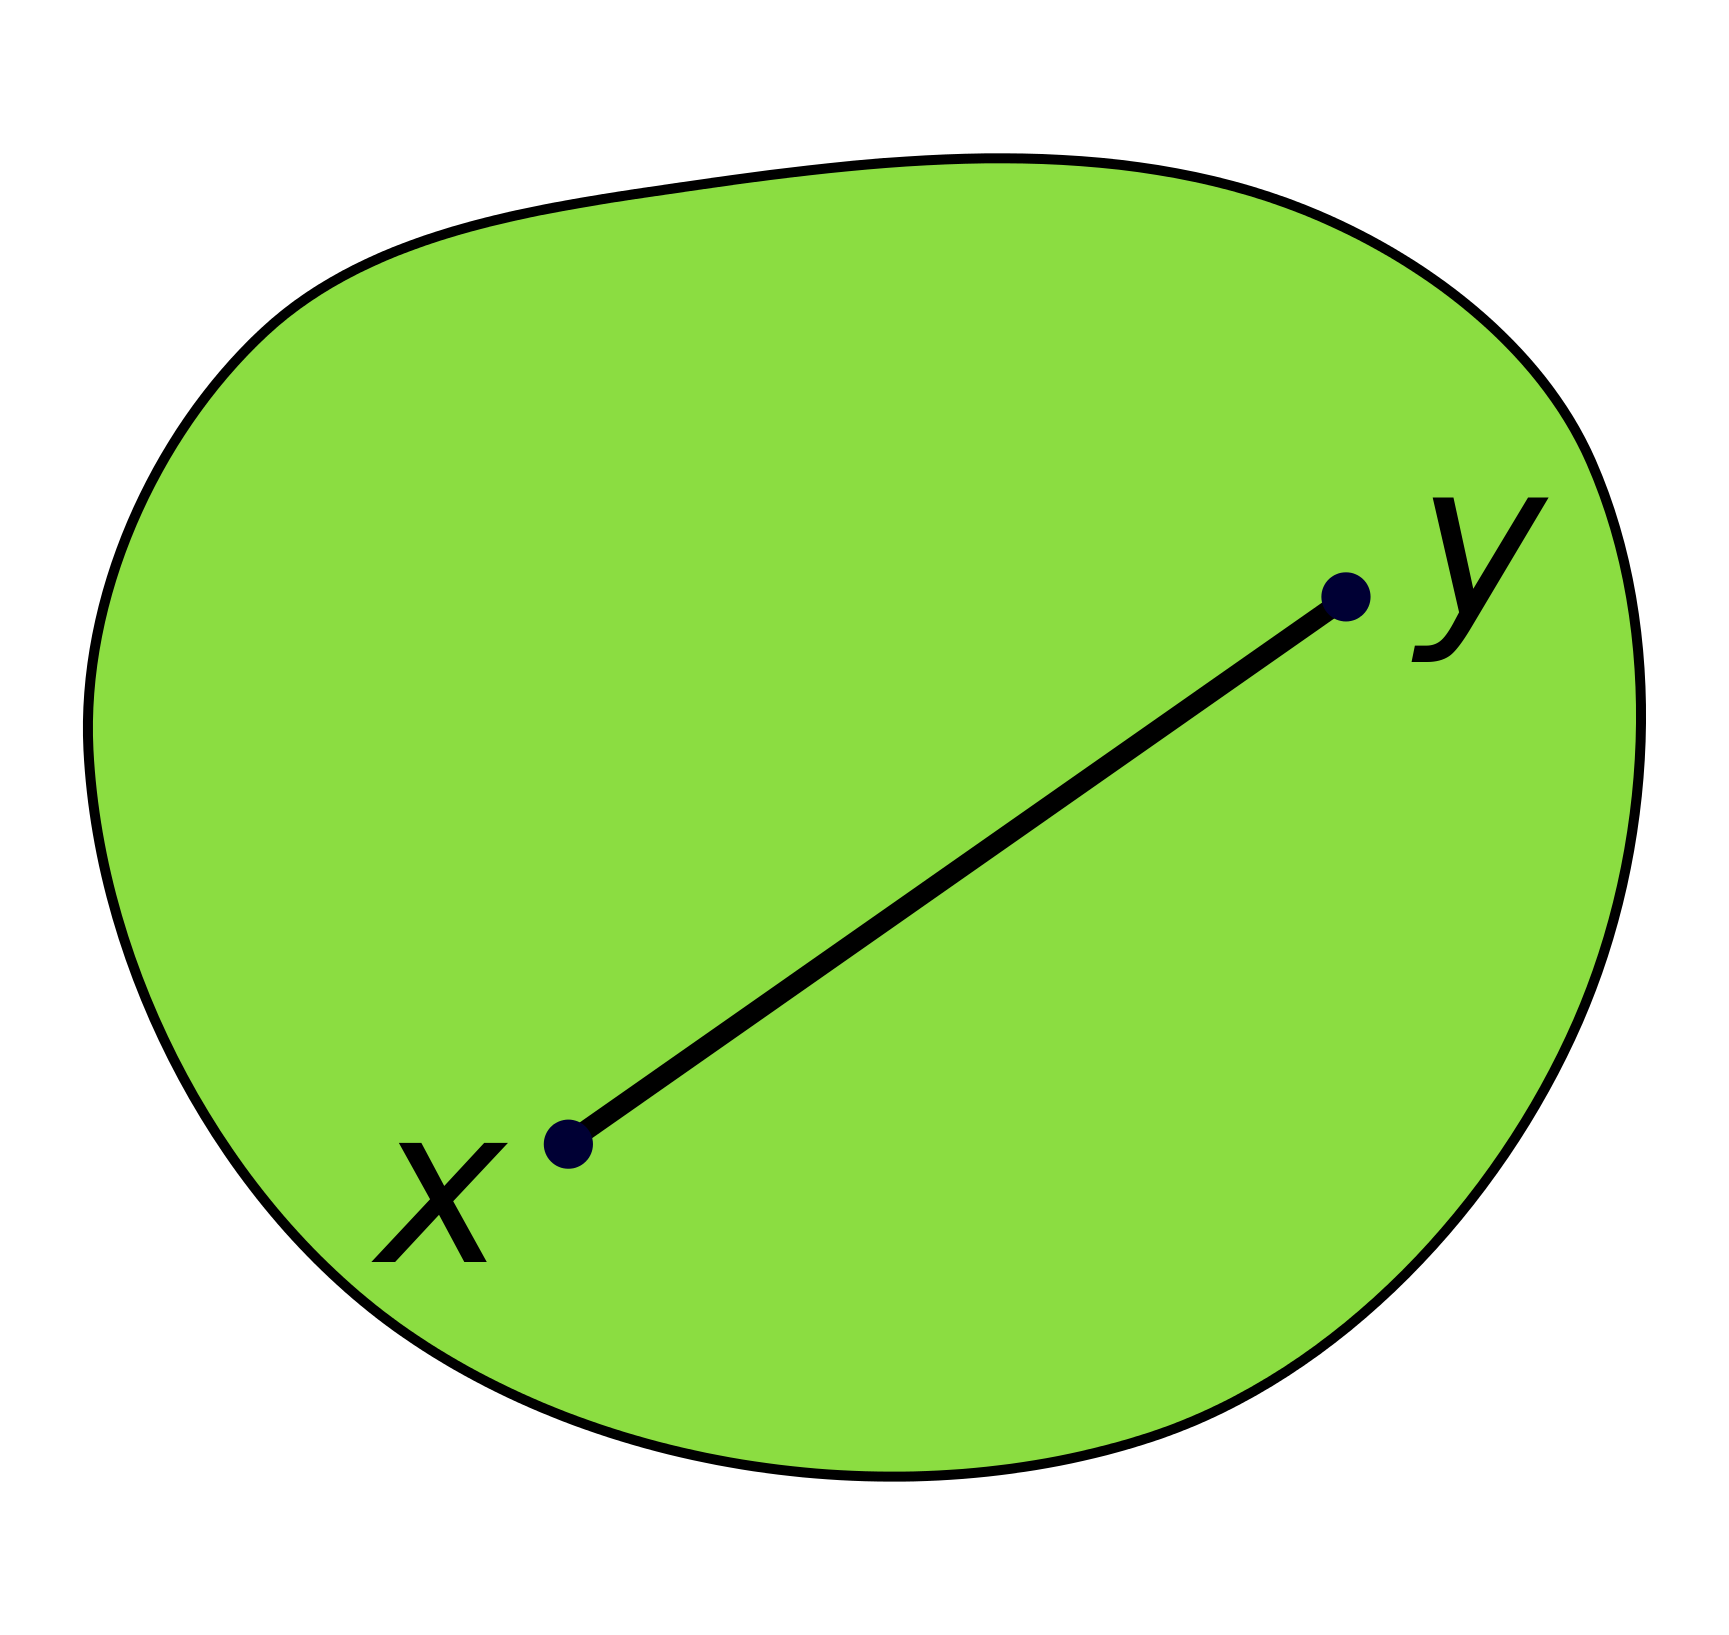
\includegraphics[width=\linewidth]{convex.png}
		\caption{Un ensemble convexe.
		Le segment de droite (noir) joignant les points $x$ et $y$
		est entièrement à l'intérieur de l'ensemble (vert).
		Comme ceci est vrai pour tous points $x$ et $y$ de l'ensemble,
		l'ensemble est convexe.}\label{fig:convex_set}
		\end{subfigure}%
		\hfill
		\begin{subfigure}[t]{.45\linewidth}
		\centering
		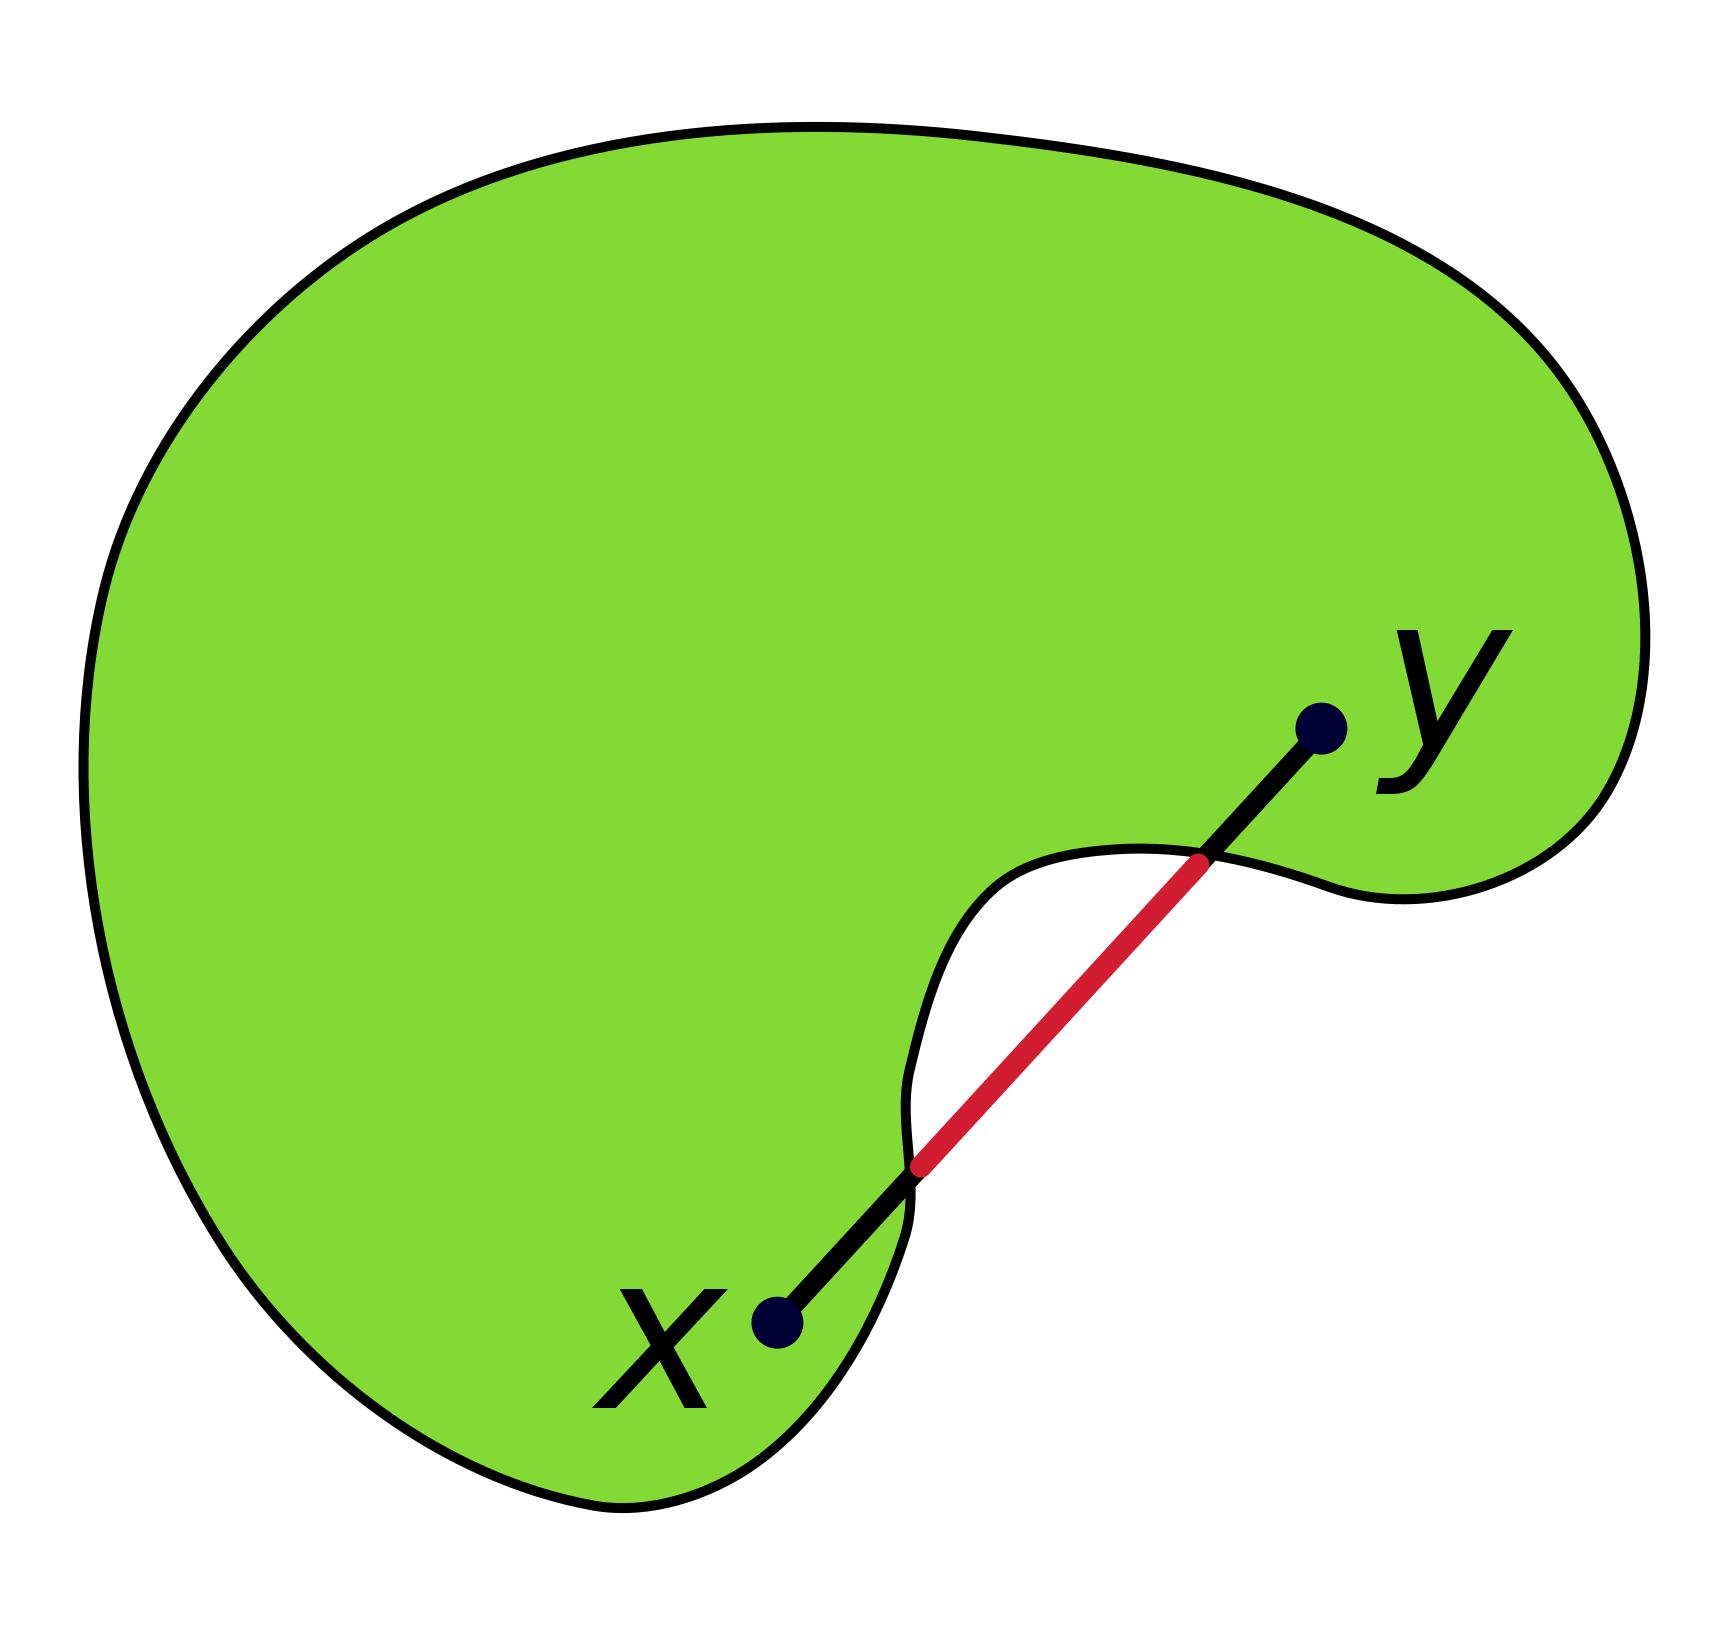
\includegraphics[width=\linewidth]{nonconvex.png}
		\caption{Un ensemble non convexe.
		Comme la partie rouge du segment de droite (noir et rouge)
		joignant les points $x$ et $y$
		est en dehors de l'ensemble (vert),
		l'ensemble est non convexe.}\label{fig:nonconvex_set}
		\end{subfigure}
		\caption{Exemples de convexité.}\label{fig:convexity}
		\end{figure}
	\end{mydef}

	\begin{mytheo}[Le demi-espace $\set{x \given a^T x \le b, a \ne 0}$ est convexe]\label{theo:demi-espace}\leavevmode
		\begin{proof}
			Si
			\[
			\left\{
			\begin{array}{c}
				a^T x \le b\,,\\
				a^T y \le b\,,
			\end{array}
			\right.
			\]
			alors a-t-on
			\[
			a^T \big(\lambda x + (1 - \lambda)y\big) \le b\,,
			\quad \forall \lambda \in \interval{0}{1}\,?
			\]

			Multiplions la première inéquation par $\lambda$,
			avec comme condition que $\lambda \ge 0$.
			Multiplions la seconde par $1-\lambda$,
			avec comme condition que $\lambda \le 1$.
			Additionnons maintenant les deux.
			On obtient alors l'inégalité suivante:
			\[
			a^T \big(\lambda x + (1 - \lambda)y\big) \le
			\lambda b + (1-\lambda) b\,.
			\]
			La partie à droite de l'inégalité se réduit facilement
			pour obtenir
			\[
			a^T \big(\lambda x + (1 - \lambda)y\big) \le b\,,
			\]
			ce qui prouve que le demi-espace est convexe.
		\end{proof}
	\end{mytheo}

	\begin{mytheo}[Convexité de l'intersection d'ensembles convexes]\label{theo:inter}\leavevmode
		Soient $\mathcal{S}_1$ et $\mathcal{S}_2$ convexes.
		Leur intersection $\mathcal{S}_1 \cap \mathcal{S}_2$
		est alors également convexe.

		\begin{proof}
			Soient $x,y \in \mathcal{S}_1 \cap \mathcal{S}_2$.

			\[
			\big(\lambda x + (1 - \lambda)y\big) \overset{?}{\subseteq} \mathcal{S}_1 \cap \mathcal{S}_2\,,
			\quad \forall \lambda \in \interval{0}{1}\,.
			\]

			Il suffit de montrer que

			\[
			\renewcommand{\arraystretch}{1.5}
			\begin{tabular}{c@{\quad}l}
				$\lambda x + (1 - \lambda)y \in \mathcal{S}_1\,,$ &
				$\lambda \in \interval{0}{1}$\\
				\multicolumn{2}{c}{et}\\
				$\forall \lambda x + (1 - \lambda)y \in \mathcal{S}_2\,,$ &
				$\forall \lambda \in \interval{0}{1}\,.$\\
			\end{tabular}
			\]
			On voit immédiatement
			que ces deux inclusions sont correctes,
			car les 2 ensembles sont convexes
			et que $x$ et $y$ appartiennent à leur intersection.
		\end{proof}
	\end{mytheo}

	\begin{mytheo}[Convexité de polyèdres]\leavevmode
		Tout polyèdre est convexe.
		\begin{proof}
			Comme un polyèdre est l'intersection
			d'un nombre fini de demi-espaces,
			en combinant le Théorème~\ref{theo:demi-espace}
			et le Théorème~\ref{theo:inter},
			on voit donc immédiatement
			que tout polyèdre est convexe.
		\end{proof}

		\begin{myrem}
			Notons que la réciproque n'est pas nécessairement vraie.
			En effet,
			prenons le contre-exemple de la boule unitaire:
			$\set{x \given \norm{x} \ge 1}\,.$
		\end{myrem}
	\end{mytheo}

\subsection{Convexité d'une fonction}

	\begin{mydef}[Convexité d'une fonction]\leavevmode
		Une fonction $f$ est dite convexe si et seulement si
		\[
		\set{(x,t) \given f(x) \le t}
		\]
		est convexe.
	\end{mydef}

	\begin{mydef}[Épigraphe d'une fonction]\leavevmode
		L'épigraphe d'une fonction $f \colon \Rn \to \R$
		est l'ensemble des points situés sur ou au-dessus
		du graphe de la fonction.

		Mathématiquement,
		\[
		\epi f = \set{(x,t) \given t \ge f(x)}\,.
		\]

		Graphiquement, on trouve ceci:

		\begin{center}
		\begin{tikzpicture}
		% this wasn't worth the effort it took...
		\begin{axis}[
			axis y line = middle,
			axis x line = middle,
			samples     = 200,
			domain      = -4.5:4.5,
			xtick       = \empty,
			ytick       = {3.7},
			yticklabels = {$t$},
			x label style={anchor=north},
			y label style={anchor=south},
			xlabel={$x \in \Rn$},
			ylabel={$f(x) \in \R$},
			xmin = -6, xmax = 6,
			ymin = -1, ymax = 6,
		]
			\addplot[name path=sqr, black, thick, mark=none, ] {sqr};
			\addplot[name path=line, gray, no markers, line width=0pt] {0.2*(4.5)^2+1.2};
			\addplot [
			color=green,
			fill=green,
			fill opacity=0.5
			]
			fill between[
			of = line and sqr,
			];
		\end{axis}
		\end{tikzpicture}
		\end{center}

		L'épigraphe est donc la partie verte du graphe.
	\end{mydef}

	Une fonction dont l'épigraphe est un polyèdre s'écrit
	\[
	f(x) = \max \left( a_i^T x - b_i \right)\,,
	\quad i \in \{1,2,\dots,n\}\,.
	\]

\subsection{Solutions}

	Prenons le système de contraintes
	\[
	\renewcommand{\arraystretch}{1.5}
	\left\{
	\begin{array}{rcl}
		x_1 & \ge & 0\,,\\
		x_2 & \ge & 0\,.
	\end{array}
	\right.
	\]
	Un point $(x_1,x_2)$ qui satisfait ces deux inéquations
	(comme par exemple $(1,1)$)
	est appelé une solution admissible de base.

	Prenons maintenant un système de contraintes différent:
	\[
	\renewcommand{\arraystretch}{1.5}
	\left\{
	\begin{array}{rcrcr}
		-x_1 & - & x_2  & \ge & -1\,,\\
		 x_1 & + & 2x_2 & \ge &  2\,.
	\end{array}
	\right.
	\]
	Le point $(0,1)$ satisfait ces deux inéquations
	de façon stricte.
	On dit que les contraintes sont ``actives'' ou ``serrées'' en $(0,1)$.
	Une solution admissible de base $x^* \in \Rn$ est dite dégénérée
	si le nombre de contraintes actives
	en $x^*$ est supérieur à $n$.

	\begin{center}
	\begin{tikzpicture}
		\begin{axis}[
			axis y line = middle,
			axis x line = middle,
			samples     = 200,
			domain      = -1:2.5,
			xtick       = {1,2},
			ytick       = {1},
			x label style={anchor=north},
			y label style={anchor=south},
			xlabel={$x_1$},
			ylabel={$x_2$},
			xmin = -2, xmax = 5.5,
			ymin = -1.5, ymax = 3,
		]
			\draw [orange, fill] (0,1) circle (2pt) node [above right] {dégénérée};
			\draw [red, fill] (2,0) circle (2pt) node [above right] {non admissible};

			\addplot[name path=c1, black, thick, mark=none, ] {1-x};
			\addplot[name path=c2, black, no markers, thick] {1-0.5*x};
			\addplot[name path=xaxis, gray, no markers, line width=0pt] {0};
			\addplot [
			color=green,
			fill=green,
			fill opacity=0.5
			]
			fill between[
			of = c1 and xaxis,
			soft clip={domain=0:1}
			];
		\end{axis}
	\end{tikzpicture}
	\end{center}

	Soit $\mathcal{P}$ un polyèdre.

	\begin{itemize}
		\item $\textnormal{$x$ est un point extrême de $\mathcal{P}$}
		\iff \nexists y,z \in \mathcal{P} \setminus \{x\} \suchthat x = \lambda y + (1 - \lambda) z\,,
		\quad \forall \lambda \in \interval{0}{1}\,.$
		\item $\textnormal{$x$ est un sommet de $\mathcal{P}$}
		\iff \exists c \suchthat c^T x > c^T y\,,
		\quad \forall y \in \mathcal{P} \setminus \{x\} \,.$
	\end{itemize}

\subsection{Variables de base et variables hors base}

	Prenons le système général suivant:
	\[
	Ax = b\,.
	\]
	On sait que

	\begin{itemize}
		\item $A$ est une matrice $m \times n$,
		\item $x$ est un vecteur colonne ($n \times 1$)
		\item et $b$ est un vecteur colonne également ($m \times 1$).
	\end{itemize}

	On a donc $m$ contraintes toujours serrées.
	Comme il faut serrer au moins autant de contraintes
	qu'il n'y a de variables,
	on serre également $n-m$ contraintes de type $x_i \ge 0$.

	Supposons sans perte de généralité que toutes les lignes de $A$
	sont linéairement indépendantes,
	c'est-à-dire que $m \le n$.

	On peut réarranger le vecteur $x$ de sorte à obtenir
	un vecteur scindé en deux selon que
	la variable $x_i$ soit égale à zéro ou pas.
	\[
	\begin{tabular}{l|c|}
		\cline{2-2}
		\multirow{3}{*}{$\xb$ ($m$ variables de base)} & \multirow{3}{*}{$\ge 0$}\\
		& \\
		& \\
		\cline{2-2}
		\multirow{5}{*}{$\xn$ ($n-m$ variables hors base)} & \multirow{5}{*}{$= 0$}\\
		& \\
		& \\
		& \\
		& \\
		\cline{2-2}
	\end{tabular}
	\]

	On doit alors scinder la matrice $A$ selon ces mêmes règles:
	\[
	A
	=
	\begin{bmatrix}
		B & N
	\end{bmatrix}\,.
	\]

	Après le choix de la base, $\xn = 0$.
	On trouve alors
	\[
	\renewcommand{\arraystretch}{1.5}
	\left\{
	\begin{array}{rcrcr}
		B \xb & + & N \xn & = & b\\
		      &   &   \xn & = & 0
	\end{array}
	\right.
	\iff
	\left\{
	\begin{array}{rcl}
		\xb & = & B^{-1} b\,,\\
		\xn & = & 0\,.
	\end{array}
	\right.
	\]

	$\xb = B^{-1} b \ge 0$ est une solution admissible de base
	si et seulement si
	$B$ a des colonnes linéairement indépendantes.
